\chapter{Theoretical Background}
\label{chap:theoretical-background}
This chapter provides an overview of the technologies and concepts referred to in subsequent chapters.
Starting with section \ref{sec:computer-networks}, essential concepts of computer communication in networks will be presented and examined, covering the concept of network layers, intercepting of communication between two parties and analysis of transferred data.
Building upon these fundamentals, section \ref{sec:internet-of-things} introduces the fields of use of \ac{IoT} applications, common architectures used today to implement them and popular protocols they make use of. Lastly, it will discuss security considerations important to \ac{IoT} applications.
After that, section \ref{sec:information-security} will provide insights into relevant concepts and the practices used and applied in information security. It covers key concepts and legal considerations, integration of information security in software development and common practices and methods involved.


\section{Design Patterns}
\subsection{Pipeline/Pipes and Filters Pattern}
%CITE: 1996 Paper Design Patterns in Software Design Patterns
\begin{figure}[h!]
    \centering
    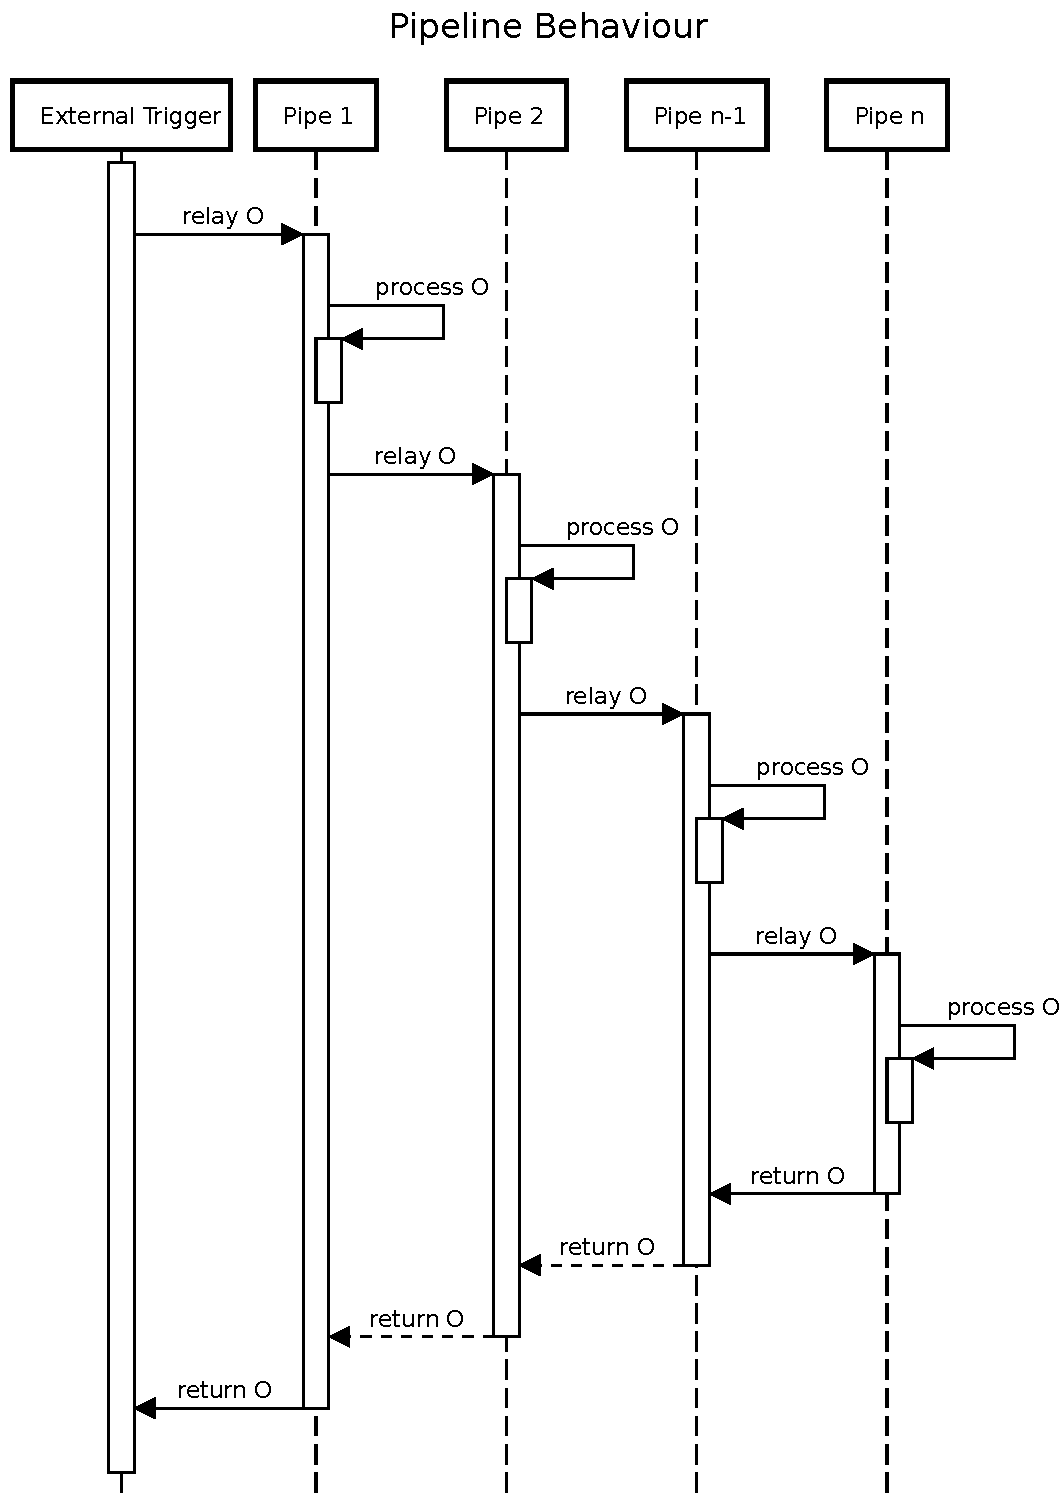
\includegraphics[width=12cm]{img/ch04/pipeline-behaviour.pdf}
    \captionof{figure}{?} % TODO
    \label{fig:dp-pipes-filters}
\end{figure}
\subsection{Abstract Factory Pattern}
%CITE: 1997 - Book - Design Patterns
\subsection{Publish-Subscribe/Observer Pattern}
%CITE: 1997 - Book - Design Patterns

\section{Computer Communication}
\label{sec:computer-networks}
\emph{TBD: OSI-Modell} %TODO
%CITE: ISO/IEC 1994
%TBD: Proxy?

\section{(Industrial) Internet of Things}
\label{sec:internet-of-things}
\subsection{Fields of Use}
%TBD: KRITIS
%CITE: 2013 - Book - BSI
%Smart Home?
\subsection{Application Architectures}
\emph{TBD: Cloud + Device}
\subsection{Common Protocols}
\label{sec:iot-common-protocols}
Building up on pre-existing network infrastructure and in order to meet requirements specific to individual fields of use and use-case scenarios, the landscape of \ac{IoT} attends with a great variety of \emph{communication protocols} (further used to refer to both transport and application protocols). This section will provide a brief overview of the working principles, use cases and history of some protocols commonly used in \ac{IoT} and \ac{IIoT} applications today.
\paragraph{\ac{HTTP}} \emph{TBD} %TODO
\ac{HTTPS}
%CITE: 1.0 https://datatracker.ietf.org/doc/html/rfc1945
%CITE: 2019 - Book - SmartInnovationsInCommunicatio - p174
\paragraph{\ac{WS}} \emph{TBD}

%CITE: https://datatracker.ietf.org/doc/html/rfc6455
%CITE: PMCE https://tools.ietf.org/html/rfc7692
\paragraph{\ac{MQTT}}
\cite{gupta_banks_2015}

\paragraph{Industrial} Modbus \ac{TCP}, Profibus/Profinet, \ac{OPC U/A}

\section{Information Security}
\label{sec:information-security}
\subsection{The CIA Triad}

\subsection{Penetration Testing}

\subsection{Man-In-The-Middle Attacks}
\ac{MITM}
%Cite: A Survey of Man In The Middle Attacks

\subsection{Tools}
There are many tools used in information security. They vary greatly in their features, field of use and maturity. The following paragraphs describe tools relevant to this thesis and the fields of use it touches.

\paragraph{Wireshark} First released in 1998, \emph{Wireshark} is a cross-platform and open-source tool used for network analysis, including \emph{network sniffing} \cite{wireshark}. It is written mainly in C, consists of more than 3,600,000 lines of C code\footnote{This number was returned by the \emph{cloc} utility run on commit \emph{c73ab16b} from 23rd May 2021 of Wireshark's GitLab source-code repository \cite{wiresharkgit}.} and features a \ac{GUI}. Although it is described as a network protocol analyser, it also supports sniffing of \ac{USB} packets. It implements a wide array of \emph{dissectors} for various protocols and allows detailed examination of network packets (as shown in figure \ref{fig:wireshark}).

\begin{figure}[h]
    \centering
    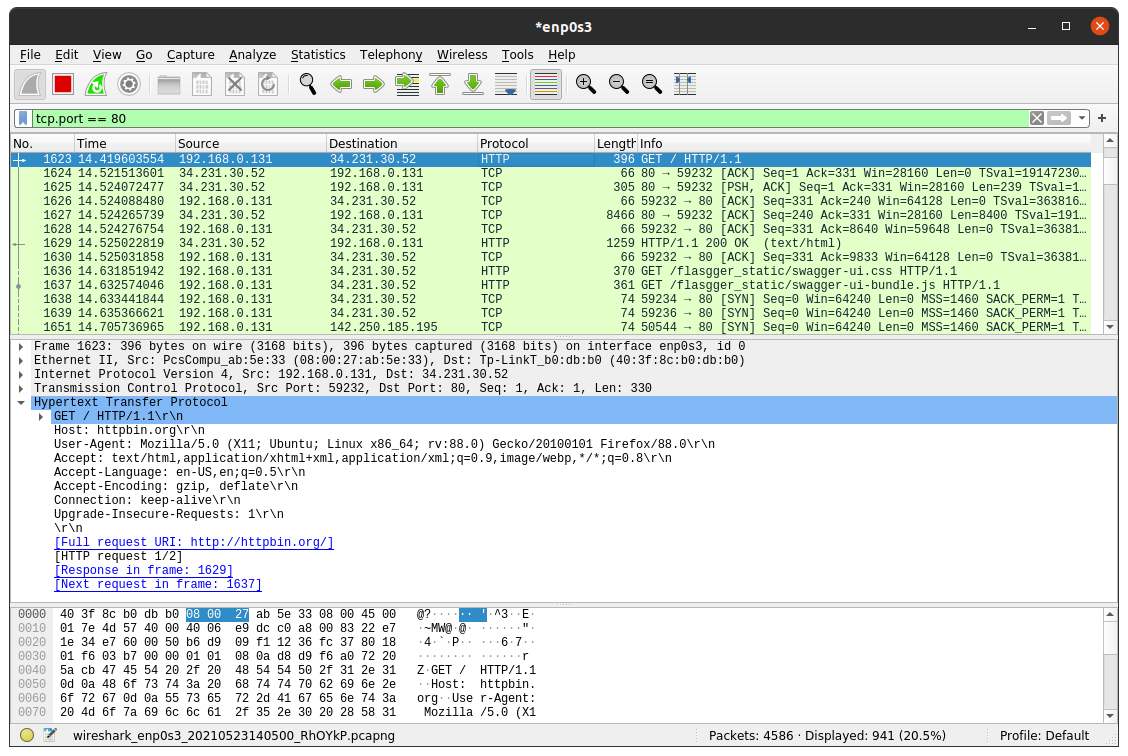
\includegraphics[width=14cm]{img/ch03/wireshark.png}
    \captionof{figure}{Screenshot of Wireshark being executed and dissecting a \ac{HTTP} $GET$ request to the site \enquote{httpbin.org}. The display-filter \enquote{tcp.port == 80} shows only packets sent to or from port 80 (e.g. \ac{HTTP} communication).}
    \label{fig:wireshark}
\end{figure}

\subsubsection{Specific \acp{MITM}}
The following tools are \acp{MITM} that support specific protocols only:
%Specific mitms:
\paragraph{Burp Suite} Developed and distributed by \enquote{PortSwigger} as a commercial product, \emph{Burp Suite} is a tool specialized for web-application testing \cite{burpsuite}. It can be used as a \ac{MITM} for \ac{HTTP} communication by configuring the operating system or browser to use its internal \ac{HTTP} server as a proxy. While it implements basic support for \ac{WS}, it is mainly used for \ac{HTTP} (and nowadays \ac{HTTPS}) and lacks support for other protocols. Aside from its internal proxy server, it also provides specialized features such as the \enquote{Repeater} which is used to send forged \ac{HTTP} requests. The freely available \enquote{Community Edition} (shown in figure \ref{fig:burpsuite}) allows use of most of the tool's features.

\begin{figure}[h]
    \centering
    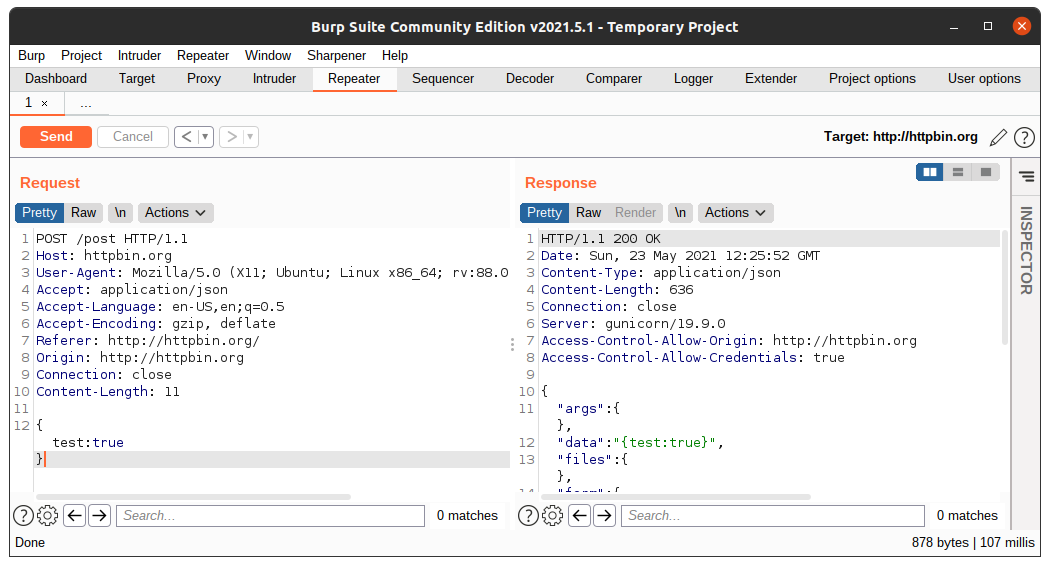
\includegraphics[width=14cm]{img/ch03/burpsuite.png}
    \captionof{figure}{Screenshot of Burp Suite being used to send forged \ac{HTTP} requests to the site \enquote{httpbin.org}.}
    \label{fig:burpsuite}
\end{figure}
\paragraph{mitmproxy} %focused on HTTP/S + WS but supports extension, largely undocumented source
\paragraph{mProxy}
\paragraph{IOXY}
%Generic
\subsubsection{Generic \acp{MITM}}
The following tools are generic \acp{MITM} that support a wide range of network protocols:
\paragraph{ettercap} While \emph{ettercap} was initially developed as a network sniffer for switched \ac{LAN}, it was gradually extended to implement a set of \ac{MITM} attacks such as \ac{ARP} spoofing and \emph{packet filtering} which allowed modifying intercepted communication \cite{ettercap}. Penetration testers can write custom filters in a scripting language to implement their own packet filtering logic. It is written in C and implements network protocols of layers 1 to 4 of the \ac{OSI} model. Thus, it does not implement application protocols.
\paragraph{bettercap} Similar to ettercap, \emph{bettercap} implements network sniffing and other features used for network analysis and discovery. However, contrary to ettercap, it aims to support a wider range of transport technologies and is described as \enquote{\emph{the Swiss Army knife for WiFi, Bluetooth Low Energy, wireless HID hijacking and IPv4 and IPv6 network reconnaissance and MITM attacks}} \cite{bettercap}. It is written in Go and features a web-interface for configuration, control and monitoring.
\paragraph{Scapy}
\paragraph{MITMf} %Built on scapy, implements some attacks and servers, not maintained anymore, superseded by bettercap 